%ब
\section{Apache Cassandra} \label{s:Background-Cassandra}

Cassandra is a distributed data storage system initially developed by Facebook
for satisfying the needs of large web applications that handle large
volumes of data~\citep{BOOK}. 
Its development has been undertaken by Apache  and it is  currently used by
many large web applications and large organisations like Facebook,  Twitter, 
Cisco,  Digg,  Reddit, and others~\citep{datastaxB}. 

Cassandra is based on the column-oriented key value data model. It stores data
as columns,  super columns,  column families and keyspaces, all of which are
explained in Section~\ref{s:key-value-data-model}. Being a distributed
system, Cassandra can run on multiple machines which are
configured to operate together and run as a single
cluster~\citep{datastax,BOOK} .
% runs as a single Java process on each machine in a cluster.
Cassandra provides the option  to work across different machines and across
multiple data centers,  even if these  are geographically
distributed~\citep{BOOK}.
The details of such a distributed nature is abstracted from  the user such that 
% the entire cluster behaves like a unified whole. and access to only
% one of the nodes is required to perform operations.
The machines in the cluster form a ring of nodes,  where
nodes are connected to each other and each node is aware of all their peers in
the cluster (Figure~\ref{f:cassandra-cluster})).


\begin{figure}[h] \centering 
	% \includegraphics[width=5cm,    height=5cm]{.  /figure/random.  jpg}
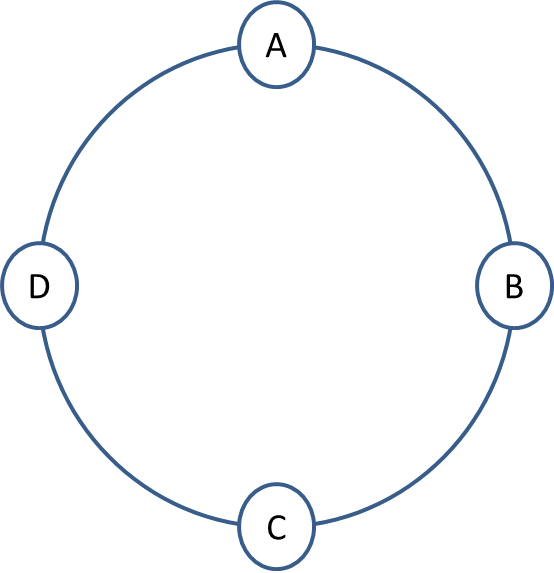
\includegraphics[width=.3\textwidth]{./figure/Background/CassandraCluster.png}
	\caption{A cluster of nodes in Cassandra}\label{f:cassandra-cluster}
\end{figure}

The nodes in a cluster communicate with each other to send their state
information at regular time intervals,  so that other nodes in the ring  know
their status~\citep{cassandra,BOOK}. Such communication
between the nodes support failure detection in Cassandra.
% helps in failure detection in Cassandra since
If a node is not active,  it fails to send or respond to messages from other
active nodes and in this way the rest of the nodes  know of its inactive state.
% Cassandra is fault tolerant and able to perform operations despite node
% failures.
% Even when some parts of the cluster are inactive, Cassandra is fault tolerant
% and contiune performing its operations. 
In the event of a node failure,
operations sent to it are not lost since another active node ensures these are
performed~\citep{cassandra}.

In such a cluster,  every node applies the same architectural features
fundamental to Cassandra,  namely,  load balancing,  replicating
and partitioning data,  failure detection mechanisms, among others.  Some of the
key architectural concepts of Cassandra are explained next. 

% Distributed system are prone to conflicts as many users could be issuing
% requests on data items from any of the nodes.  Any distributed system should
% carefully consider conflict resolution and adopt design approaches which would
% resolve such conflicts efficiently.  Conflicts arise either at read or write
% operations. 
% The design approach should either make the system resolve such conflicts either
% during one of these operations,  deciding the system be either readable at all
% times or writable.  Cassandra optimises its performance by adopting the design
% approach of resolving conflicts during read operations,  making Cassandra always
% writable. 



\subsection{Architecture} \label{ss:Background-Cassandra-Archi}
Cassandra adopts many of its  architectural concepts from other popular
distributed key-value data storage systems on the cloud,  like Google's Bigtable
and Amazon's Dynamo~\citep{ycsb,Dynamo}.  Over time, these adopted concepts
evolved and developed new features,  some of which became specific to Cassandra's
architecture. Some of these  concepts are, peer-peer distribution model, data
partitioning, eventual consistency, among others. These  concepts gave Cassandra
  features such as elastic scalability,  fault tolerance, high availability and
high performance.
% Cassandra's architecture involves many sophisticated and complex theoretical
% as well as mathematical concepts,
% Following are some of the key architectural concepts of Cassandra.
% Discussing every concept is beyond the scope of this research.



\subsubsection{Peer-Peer Distribution Model}
% Generally,  in traditional distributed
% \acp{DBMS},  nodes in a cluster are configured to have different
% responsibilities and roles where some or one of the nodes is a master and others
% are slaves.  Such a centralised configuration improves reading data,  as data can
% be read from any of the slave nodes,  but write requests are always sent to the
% master node.  This model thus puts a lot of additional load on the master and
% also is prone to failure if the single master node is offline.  However, 
Cassandra is a decentralised system  where all the nodes are considered equal
or identical (i. e.  nodes are peers) in sharing responsibilities and performing
operations,  without any  master or slave nodes~\citep{datastaxB,BOOK}. 
This model provides high data availability since failure
of a node does not affect the service of the cluster  because other
nodes carry out the same operation. 
% Moreover,  when new nodes are added to a cluster there is no additional task of
% delegating responsibilities or roles since all the nodes have the same
% responsibilites. 

% The nodes in a cluster communicate with each other to send their state
% information at regular time intervals,  so that other nodes in the ring can know
% their status (\todo{cite Cassandra paper}).  This helps in failure detection in
% Cassandra since if a node is not active it fails to send or respond to  messages
% from other active nodes and in this way the rest of the nodes  know of its
% inactive state.  In the event of a node failure,  another active node  performs
% the operations in order to ensure that  operations that were sent to a failed
% node are not lost (\todo{cite Cassandra papers}). 
% The recepient node  creates a small hint message with the information about
% the operation so that it can give the hint to the failed node once it is
% alive again and this feature is called hinted handoff. 

\subsubsection{Data Partitioning}
Cassandra partitions data between the nodes in a cluster  so that data items
from overloaded or failed nodes are assigned to other nodes or new nodes.  For
this,  Cassandra uses consistent hashing where data items are hashed on its key.
After hashing the key, the data items are assigned to the node whose
position in the ring is larger than the hashed value of the key~\citep{BOOK}.
% used by Amazon's Dynamo to partition data over the nodes. (\todo{DeCandia et
% al. (2007)}). 
% \begin{figure}[h] \centering %\includegraphics[width=5cm,    height=5cm]{. 
% /figure/random.  jpg}
% 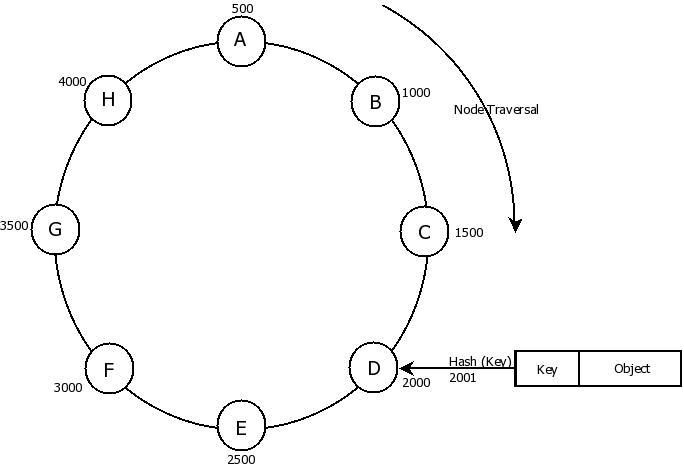
\includegraphics[width=. 6\textwidth]{. /figure/Cassandra/Consistent-hashing-Cassandra. png}
% \caption{Consistent hashing in Cassandra}\label{f:consistent hashing}
% \end{figure}
Data partitioning makes Cassandra elastically scalable since the load is
balanced and distributed in the cluster  irrespective of addition or removal of
nodes~\citep{BOOK,cassandra}. 
% Additionally,  in Cassandra better performing nodes are assigned multiple
% points in the ring,  making them virtual nodes and these nodes are assigned
% workloads from failed nodes or overloaded nodes. 

\subsubsection{Replication strategy} In order to ensure high data availability
irrespective of failures,  Cassandra uses a replication strategy where every
data item is replicated across a number of nodes.  Applications can set the
level of replication to suit its requirements,  that is, the replication factor
is set to the number of nodes on which the application wants to create
replicas~\citep{BOOK,cassandra}.  The
replication factor tells the cluster how many copies to create of a single data item.
Setting the replication factor to a large number would help in higher
consistency of data items,  but replicating data items to a large number of
nodes  can adversely affect the performance.

Once data items are partitioned and assigned to a node,  these are
replicated onto other nodes and a list of the nodes responsible for storing the
data items are maintained.  Thus, every node in the cluster knows which nodes
are responsible for a data item~\citep{BOOK,cassandra}.
Such a replication strategy makes data highly available  since data items can
be accessed from any node in a cluster regardless of node failures.  
% Since all
% the nodes  know which peer node is responsible for a data item,  
% routing requests to the correct nodes. 



\subsubsection{Eventual Consistency}
% As mentioned previously,  Cassandra opts for '\texttt{A}' and '\texttt{P}' of
% the CAP theorem and allows users to determine the level of consistency they
% prefer.  This consistency level tells the cluster how many replicas should
% acknowledge operations done on them,  for the replicas to be considered
% consistent and up to date.  Low consistency levels are considered better for
% performance as higher consistency levels involve more time since nodes have to
% wait to receive acknowledgements from more replicas.
% Letting the users decide the consistency level and replication factor means
% the tradeoff between consostency and performnace is detemined by the users.
In any strongly consistent  \acp{DBMS}, data items immediately reflect the new
values upon an insert or update operation. However, Cassandra uses the eventual
consistency model where replicas do not agree to the most recent value
immediately but will do so eventually. This is because the new values are
propagated to all the replicas in a cluster in an asynchronous
way~\citep{Tai,ycsb,henry,Vogel}.
% Eventual consistency provides Cassandra high scalability because any write or
% update operation  reaches all the replicas irrespective of the number of
% nodes in a cluster.
% Thus,  all replicas would be consistent eventually after a certain period of
% time, generally a small number of milliseconds \todo{cite book}.
% This is unlike strict consistency models  run on single nodes,  where a read
% operation always returns the most update values.
% In distributed systems like Cassandra,  several machines are used concurrently
% by many users leading to various conflicts,  which makes a weaker form of
% consistency like eventual consistency  ideal (\todo{cite BOOK and marked
% papers}).

 
\subsection{Write and Read Operations}
\label{ss:Background-Cassandra-Operations} 
In order to write data into Cassandra column families,  a write request is sent
to a random node in the cluster,  which acts as a proxy node and replicates the
data in the cluster~\citep{datastax,BOOK,cassandra}.
The number of nodes on which data is to be replicated can be changed to suit the
application requirements. Moreover, these nodes can be in the same data centre
and other data centres.

		

When a read request is issued to a node,  it acts as a proxy node and forwards
the request to all the other nodes in the cluster.
These nodes return their copy of the data item to the proxy node and the proxy
node  checks the versions of the replicas and sends the latest replica to the
user~\citep{datastaxRead}.   If the replicas received from a node are not
consistent with other replicas, a read repair is performed on the node
with the outdated replicas.  This means that the nodes with outdated replicas
are sent a write operation with the latest data.
Thus,  data consistency is maintained whenever conflicting versions of data
items are found.



